%%%%%%%%%%%%%%%%%%%%%%%%%%%%%%%%%%%%%%%%%
% SLAB Report Template
% Version 1.0
% Adam W Koenig, February 2014
%%%%%%%%%%%%%%%%%%%%%%%%%%%%%%%%%%%%%%%%%

\documentclass{article}

\usepackage{mhchem} % Package for chemical equation typesetting
\usepackage{siunitx} % Provides the \SI{}{} command for typesetting SI units
\usepackage[top=1.5in, bottom=1.5in, left=1.5in, right=1.5in]{geometry}
\usepackage{fancyhdr}
\usepackage{multirow}
\usepackage{setspace}
\usepackage{float}
\usepackage{amsmath}
\pagestyle{fancy}
\headheight 32pt

\usepackage{graphicx} % Required for the inclusion of images

%\setlength\parindent{0pt} % Removes all indentation from paragraphs

\renewcommand{\labelenumi}{\alph{enumi}.} % Make numbering in the enumerate environment by letter rather than number (e.g. section 6)

%\usepackage{times} % Uncomment to use the Times New Roman font
\newcommand\norm[1]{\left\lVert#1\right\rVert} %create norm command


%%%%%%%%%%%%%%%%%%%%%%%%%%%%%%%%%%%%%
% Title Page
%%%%%%%%%%%%%%%%%%%%%%%%%%%%%%%%%%%%%

\lhead{
\includegraphics[width=2cm]{SLABlogo.png}}
\rhead{
\includegraphics[width=2cm]{AAlogo.jpg}}

\begin{document}

\begin{titlepage}
    
\includegraphics[width=6cm]{SLABlogo.png}
    \hskip1cm
    
\includegraphics[width=6cm]{AAlogo.jpg}
    \centering
    \vfill
    {\Huge\bf Analysis of GPS Interface Outputs and Orbit Estimation Using PRISMA Flight Data}\\
    \vskip2cm
    {\Large Adam M. Resnick\\
    \vskip.25cm
    August 2014\\
    \vskip.25cm
    Advisor: Professor Simone D'Amico\\
    \vskip.25cm
    Version 0.1\\}
    \vfill
\end{titlepage}

%%%%%%%%%%%%%%%%%%%%%%%%%%%%%%%%%%%%%
% Abstract
%%%%%%%%%%%%%%%%%%%%%%%%%%%%%%%%%%%%%

% \begin{abstract}
% Abstract text
% \end{abstract}

%%%%%%%%%%%%%%%%%%%%%%%%%%%%%%%%%%%%%
% TOC
%%%%%%%%%%%%%%%%%%%%%%%%%%%%%%%%%%%%%

\tableofcontents{}
\newpage

%%%%%%%%%%%%%%%%%%%%%%%%%%%%%%%%%%%%%
% Acronyms
%%%%%%%%%%%%%%%%%%%%%%%%%%%%%%%%%%%%%

{\Large\bfseries Acronym Definitions}\\
\addcontentsline{toc}{section}{Acronym Definitions}

\begin{description}
\item[CNR] Carrier-to-Noise Ratio
\item[ECEF] Earth-Centered Earth-Fixed Reference Frame
\item[ECI] Earth-Centered Inertial Reference Frame
\item[GIF] GPS Interface
\item[GPS] Global Positioning System
\item[GMST] Greenwich Mean Sidereal Time
\item[PRN] Pseudo-Random Noise Code (GPS Satellite Identifier)
\item[RTN] Radial Tangent Normal Reference Frame
\item[SNR] Signal-to-Noise Ratio
\item[SV] Space Vehicle (a GPS Satellite)
\item[UTC] Coordinated Universal Time
\end{description}
\newpage

%%%%%%%%%%%%%%%%%%%%%%%%%%%%%%%%%%%%%
% Report Body
%%%%%%%%%%%%%%%%%%%%%%%%%%%%%%%%%%%%%

\section{Overview}
PRISMA is a satellite formation flight technology demonstrator mission composed of two satellites. Mango is the main satellite and Tango is the target satellite. These are sometimes referred to as the chief and deputy satellites, respectively. GIF (GPS Interface) is the module from the PRISMA GNC flight software which reads the data from the GPS receivers of both the Mango and Tango spacecraft and outputs the navigation solutions. However, GIF cannot directly read the winmon file format of the GPS receiver. Thus, the GPS data file is read by the winmon\textunderscore reader module, which feeds GIF the memory address and length of the appropriate winmon message.

Both GIF and winmon\textunderscore reader have been embedded in Simulink through the use of S-Functions, allowing Simulink to run the C/C++ code. A Simulink model has been built around this, reading in a winmon file from PRISMA, and working with the navigation solution provided by GIF. The navigation solution is provided in an Earth-centered Earth-fixed (ECEF) frame, and is rotated to an Earth-centered inertial frame (ECI), and then to the radial, tangent, normal frame (RTN) typically used for spacecraft formation flight. 

This simulation has been run with GPS data from a 17 hour period on March 17, 2011 starting at 09:00:00 UTC. 

\section{Analysis of GIF's Output}
\subsection{Overview of GIF Outputs}
GIF provides 11 outputs. The first is DLR\textunderscore TM\textunderscore GIF, which has 5 elements. The first two are each 7 bit arrays describing the status of Mango and Tango, respectively. The third and fourth elements, respectively, are the number of GPS space vehicles (SVs) tracked by Mango and Tango. The final element is the number of commonly tracked SVs. This output can be seen below in Figure~\ref{fig:common} over the simulation time interval.

\begin{figure}[H]
    \centering
    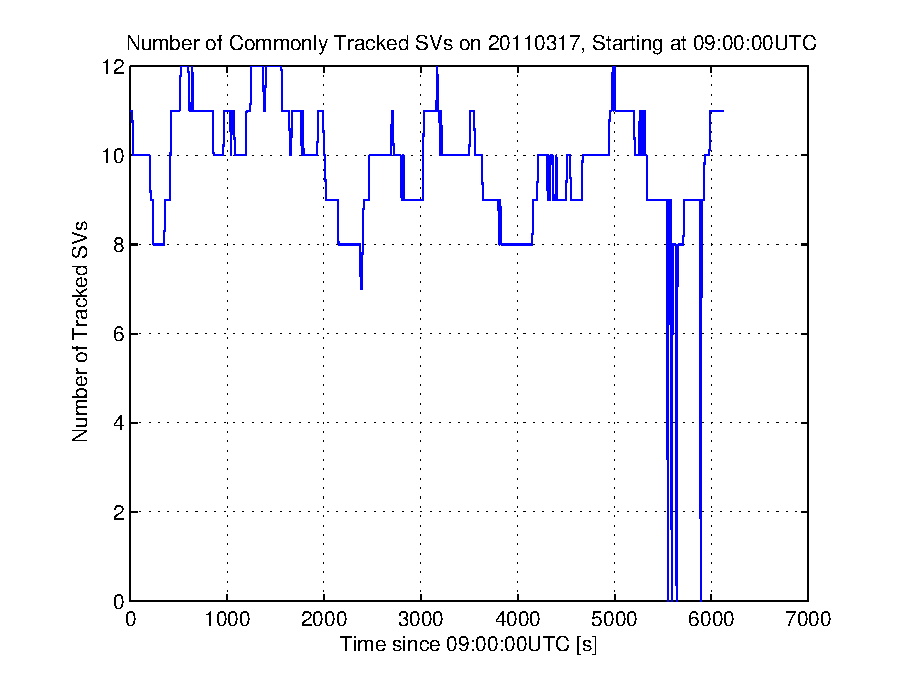
\includegraphics[width=10cm]{commonSVs.eps}
    \caption{The number of commonly tracked SVs over the simulation period.}
    \label{fig:common}
\end{figure}


The next output is TC\textunderscore DLR\textunderscore GPS\textunderscore MAIN. This provides transmit ephemeris (TE) messages for Mango. These are issued for those PRNs where observations have been collected, but no ephemeris is available. TE messages can be enabled or disabled in GIF through the TC\textunderscore DLR\textunderscore GIF input. The DLR\textunderscore GPS\textunderscore TARGET output provides the same information for Tango. 

The GPS\textunderscore Status\textunderscore MAIN and GPS\textunderscore Status\textunderscore TARGET outputs are each 7 bit arrays providing information about the status of the GPS receivers for Mango and Tango, respectively. The array contains bits that reflect the existence of a valid navigation solution, valid checksums with the receiver's messages and recent arrival of messages.

TSync is a two element output that provides GPS seconds and fractional seconds (in $\mu$s) from the initial epoch. This data would be used by the operators for on-board time synchronization. DLR\textunderscore GPS\textunderscore Obs\textunderscore Time is similar to TSync. It provides the GPS measurement epoch for use in later flight software modules.

DLR\textunderscore GPS\textunderscore MAIN\textunderscore OBS is an 81 element output containing the latest navigation solution for Mango. It contains the latest GPS raw data set common to both Mango and Tango. If there is no common time tag, the last data epoch of Mango and Tango will be taken individually. This output contains the GPS-UTC offset in seconds, the PRN number being tracked by each of the receiver's 12 channels and the position and velocity (in \si{\meter} and \si{\meter\per\second}, respectively). It also provides the C/A pseudorange [\si{\meter}], integrated carrier phase [\si{cycles}], range rate [\si{\meter\per\second}] and carrier-to-noise ratio (CNR) [\si{dBHz}] for each channel. DLR\textunderscore GPS\textunderscore TARGET\textunderscore OBS provides the same information for Tango. 

The GPS CNR over the chosen simulation period for channel one is shown in Figure~\ref{fig:CNR}. Over this period, channel one locks on to four separate PRNs. The minimum CNR to be considered valid is 35 \si{dBHz}. The CNR is important as it directly relates to the signal-to-noise (SNR) ratio of the GPS signals. If the CNR is too low, the receiver will not be able to lock onto a GPS SV.

\begin{figure}[H]
    \centering
    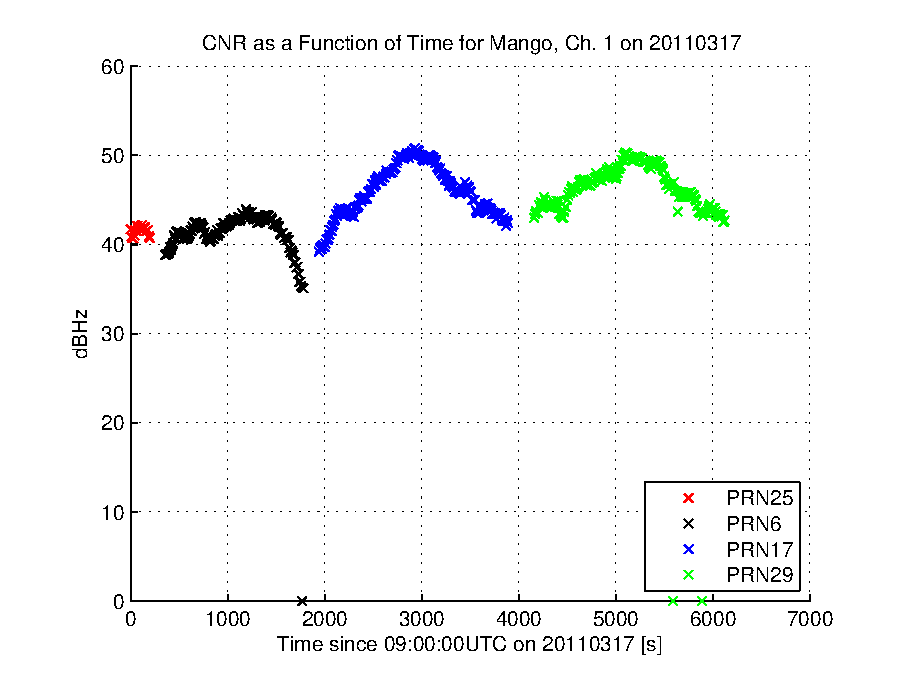
\includegraphics[width=10cm]{CNR.eps}
    \caption{The carrier to noise ratio for Mango's channel one over the simulation time. Note that four PRNs are shown over this period on this channel.}
    \label{fig:CNR}
\end{figure}

DLR\textunderscore GPS\textunderscore EPH is a 992 element output which provides a complete set of GPS ephemerides for each of the 32 PRNs in the GPS constellation.

DLR\textunderscore GPS\textunderscore UTC provides the integer offset between GPS time and UTC in seconds. This output is derived from the GPS receiver data.

\subsection{Processing GIF's Outputs}
The navigation solution output by GIF is the position [\si{\meter}] and velocity [\si{\meter\per\second}] in an ECEF frame. This navigation solution is then converted to an ECI frame. To accomplish this, the GPS week and seconds of the week are converted to a modified Julian date $MJD$. Greenwich mean sidereal time is approximately computed using [CITE AA279 SPRING LECTURE 6]
\[\theta(MJD) = 280.4606^{\circ} + 360.9856473^{\circ}(MJD-51544.5) \]
After converting this to radians, we then form the rotation matrix 
\[R_{ECI->ECEF} = \begin{pmatrix}
    cos(\theta) & sin(\theta) & 0\\
    -sin(\theta) & cos(\theta) & 0\\
    0 & 0 & 1
  \end{pmatrix} \]
noting
\[ R_{ECEF->ECI} = (R_{ECI->ECEF})^T \]
we compute 
\[ \vec{X}_{ECI} = R_{ECEF->ECI}\vec{X}_{ECEF} \]
where $\vec{X}$ contains a $(x,y,z)^T$ position fix.

The absolute orbits of Mango and Tango are then plotted in the ECI frame in Figure~\ref{fig:ECI}.

\begin{figure}[H]
    \centering
    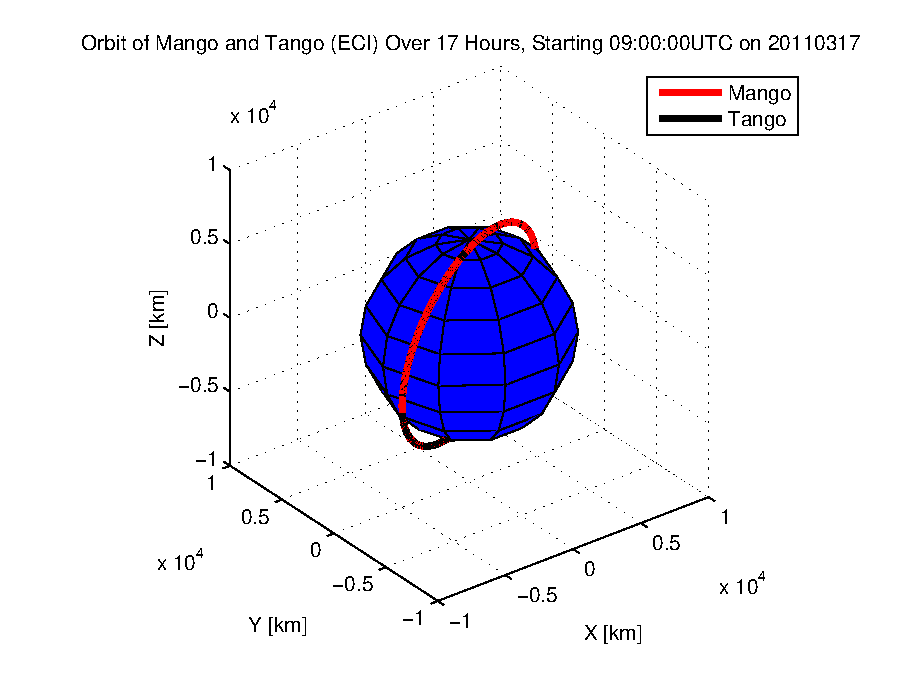
\includegraphics[width=10cm]{ECI_orbit.eps}
    \caption{The orbits of Mango and Tango in inertial space over the simulation time period.}
    \label{fig:ECI}
\end{figure}

To transform the velocity between frames, we note that
\[\omega = \begin{pmatrix}
                    0\\
                    0\\
                    \theta(MJD) 
            \end{pmatrix} \]
and then compute the ECI velocity as
\[\vec{V}_{ECI} = R_{ECEF->ECI}(\vec{V}_{ECEF} + \vec{\omega} \times \vec{X}_{ECEF}) \]

The transformed velocity of Mango can be seen in Figure~\ref{fig:vel}.
\begin{figure}[H]
    \centering
    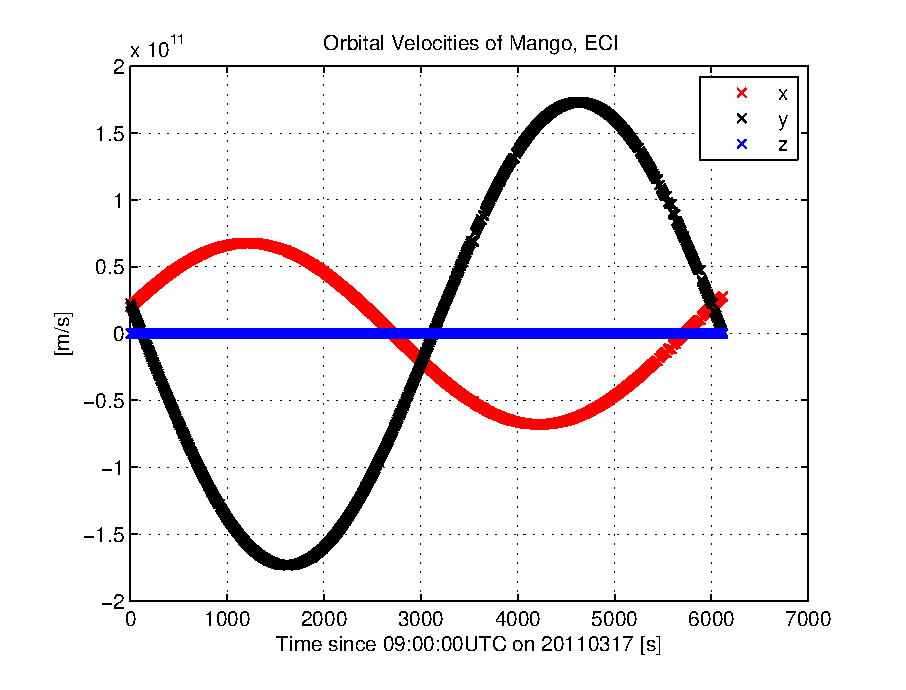
\includegraphics[width=10cm]{mainVelocity.eps}
    \caption{The X,Y and Z components of Mango's velocity in inertial space over the simulation period.}
    \label{fig:vel}
\end{figure}

As PRISMA is a formation flight mission, we are naturally interested in the position of Tango relative to Mango. This is typically viewed in a Radial, Tangent, Normal (RTN) frame moving with Mango. To map the positions from inertial space to the RTN frame, we first compute the $R$,$T$,$N$ unit vectors in the ECI frame. 
\[\hat{R}_{ECI} = \frac{\vec{X}_{ECI}^{Mango}}{\norm{\vec{X}_{ECI}^{Mango}}}\]
\[\hat{N}_{ECI} = \frac{\vec{X}_{ECI}^{Mango} \times \vec{V}_{ECI}^{Mango}}{\norm{\vec{X}_{ECI}^{Mango} \times \vec{V}_{ECI}^{Mango}}} \]
\[\hat{T}_{ECI} = \hat{N}_{ECI} \times \hat{R}_{ECI} \]
We then form the rotation matrix
\[R_{ECI->RTN} = (\hat{R}_{ECI},\hat{T}_{ECI},\hat{N}_{ECI})^T \]
The relative distance in the RTN frame can then be computed as 
\[ \vec{D}_{RTN} = R_{ECI->RTN}(\vec{X}^{Tango}_{ECI} - \vec{X}^{Mango}_{ECI})\]
This is shown in Figure~\ref{fig:RTN}.
\begin{figure}[H]
    \centering
    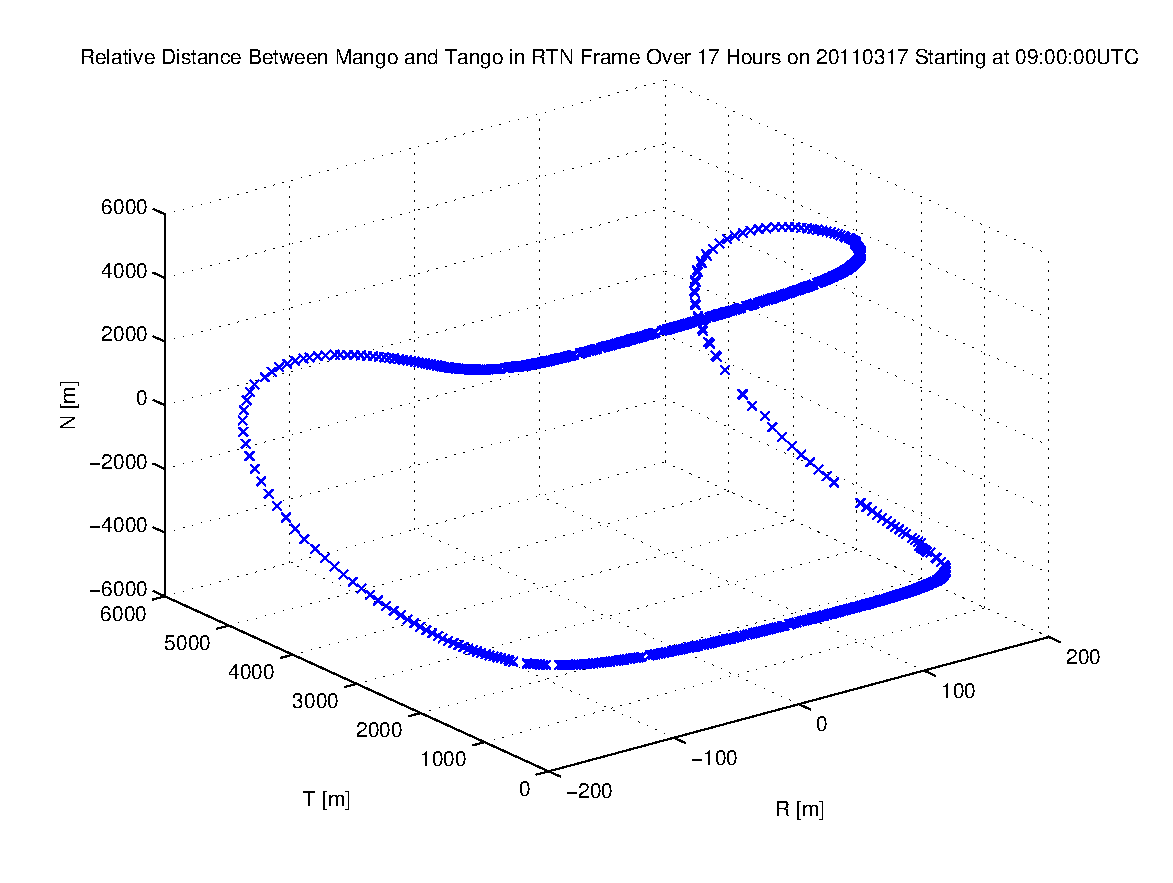
\includegraphics[width=10cm]{RTN.eps}
    \caption{The relative position of Tango with respect to Mango during the simulation period.}
    \label{fig:RTN}
\end{figure}

\section{Coarse Orbit Estimation}
TODO

%%%%%%%%%%%%%%%%%%%%%%%%%%%%%%%%%%%%%
% Bibliography
%%%%%%%%%%%%%%%%%%%%%%%%%%%%%%%%%%%%%

\bibliographystyle{unsrt}
\addcontentsline{toc}{section}{References}
\bibliography{CameraBib}


\end{document}